\documentclass{article}
\usepackage{pgfplotstable}
\usepackage{pgfplots}
\usepackage{graphicx}
\usepackage{csquotes}
\usepackage[giveninits=true]{biblatex}
\usepackage{authblk}
\usepackage{hyperref}
\usepackage{tabularx}
\usepackage{caption}
\usepackage{wrapfig}
\usepackage{fancyvrb}
\usepackage{lipsum}
\usepgfplotslibrary{units}
\pgfplotsset{compat=1.16}

\begin{document}




\title{PDE Solvers for the Laplace's Equation}
\author{Fredrik Öberg \\ \href{mailto:fobe@kth.se}{fobe@kth.se}}
\affil{Examiner: Prof. Vladimir Vlassov}
\affil{KTH Royal Institute of Technology, Sweden}
\date{\today}
\maketitle


\newpage
\tableofcontents
\newpage

\section{Introduction}
This paper is written as a part of the examination of the course ID1217 Concurrent Programming 
itself part of the operations of KTH Royal Institute of technology. The course provides knowledge about the core concepts and techniques for concurrent programming - both process oriented and multithreaded. The course also provides an overview of principles of distributed and parallel programming and is intended to give knowledge and skills in process-oriented programming. 
The students of the course had the choice of several project to implement where the aim was to practice in development, implementation, and evaluation of concurrent and distributed programs/systems. The chosen project – and the theme of this paper - was to create sequential partial differential equation(PDE) solvers for the Laplace’s equation as well as optimizing them for performance. The task was also to learn how to use parallel programming with the intent to increase the implementations performance while keeping their correctness and to conduct timing experience to analyze the performance of the different versions and compare their performance variations.

\section{Background}\label{programs}

A computational model is a mode of discovery which uses computers to simulate phenomena and to address questions about how huge events like nuclear fusion, weather, stellar evolution etc. could evolve from a given premise. Three fundamental techniques are used regularly when computing these models: grid computations, particle computations and matrix computations where grid computations(the focus of this paper) arise in numerical solutions to PDEs and in other applications(image processing for example) that divide a spatial region into a set of points. 

Laplace’s equation is an elliptic second order PDE were given a spatial region and values for points on the boundaries of the region the goal is to approximate the steady state solution for points of the interior. This can be done covering the regions with an evenly spaced grid of points and a set of interior points initialized to some value. The steady state values of the interior points are then calculated through repeated iterations of mathematical procedures. On each of those iterations is the new value of a point set to the combination of the old and/or new values of neighbouring points and terminates either after a given number of iterations or when every new value is within some acceptable difference of every old value – a value often called epsilon. Two iterative methods for solving Laplace’s equation are sequential Jacobi iteration as well as multigrid iterations and these are the PDE solver methods forming the basis of the implementations this paper is based on. 

\begin{wrapfigure}{r}{0.42\textwidth}
    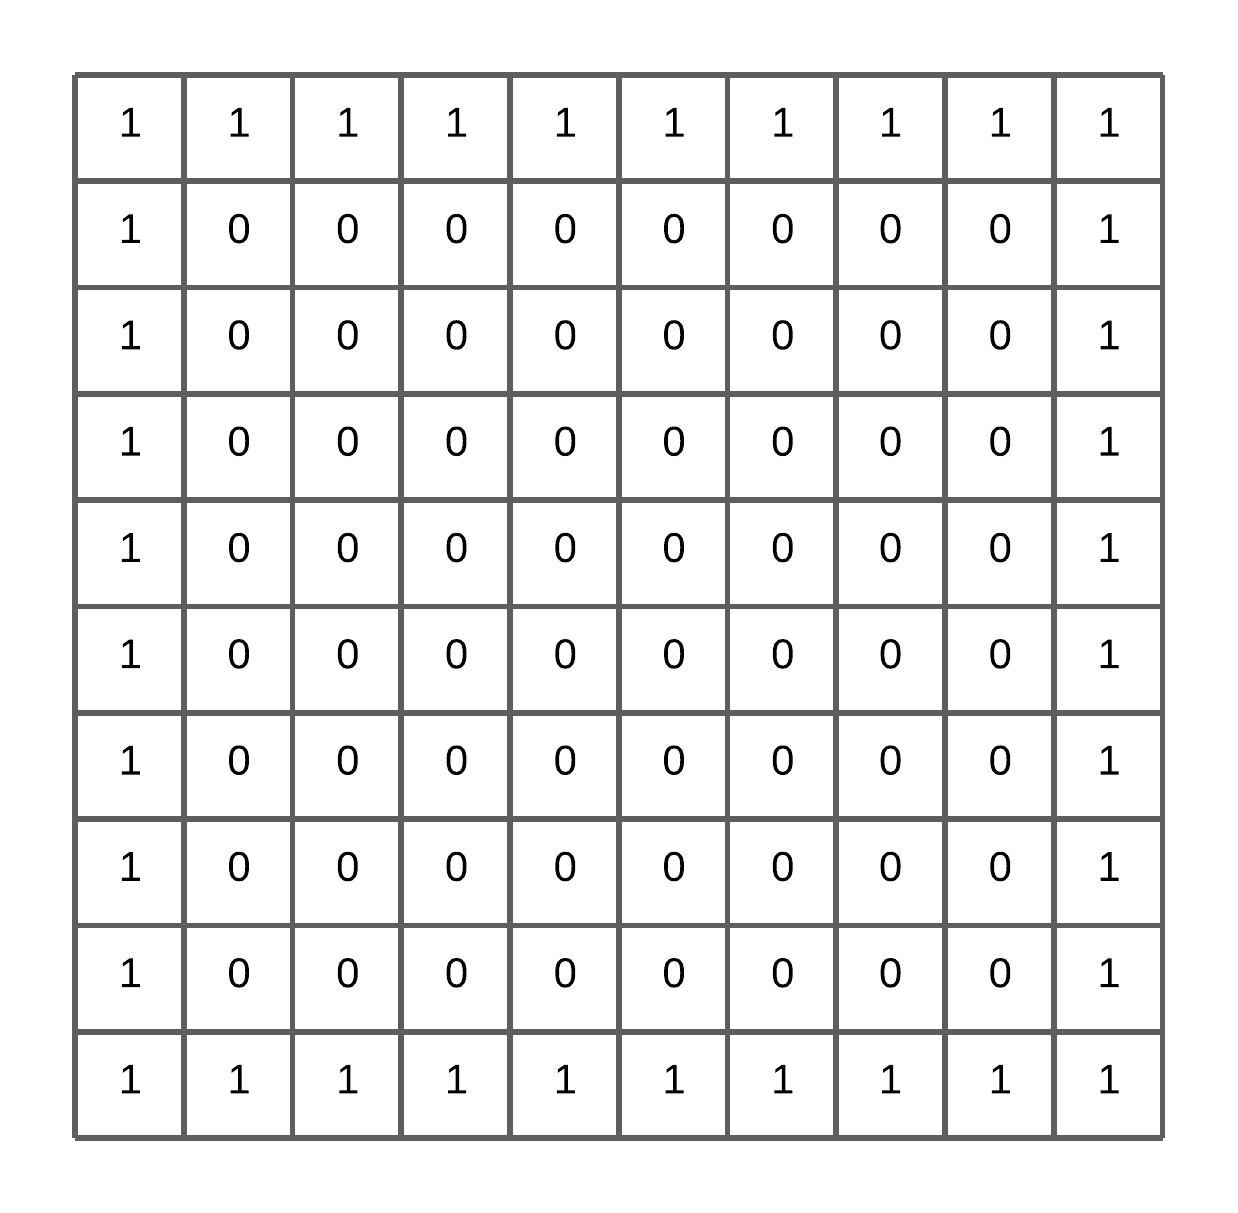
\includegraphics[width=0.4\textwidth]{../images/grid.png}
    \caption{Initial grid}
    \label{grid}
\end{wrapfigure}
\newpage

\section{Programs}\label{programs}

In Jacobi iteration is the new value of each grid-point set to the average of the old values of the four points left, right, above, and below it. These calculations are performed in a loop which repeats until the computation terminates. This is implemented by creating an N*N square-grid surrounded by a square of boundary points where the boundary values are initialized to one and the interior grid points to zero(see Figure 1). Instead of terminating when reaching an acceptable value of epsilon is the Jacobi iterations of the implementations terminated after an M number of iterations. The epsilon value is then calculated after the iterations are terminated with the intent of not letting the program execute for an unpredictable amount of time. Two grids were created and used in the implementation since the new values calculated needed to be stored in a temporary grid to not overwrite old values still needed for future calculations. How this is implemented can bee seen in the following pseudo code:


\begin{verbatim}

        for [index = 0 to ITERATIONS by 2]{
            for [i = 1 to GRIDSIZE j = i to GRIDSIZE]
                new[i,j] = (grid[i-1,j] + grid[i+1,j] +
                 grid[i,j-1] +  grid[i,j+1]) * 0.25
	
            for [i = 1 to GRIDSIZE j = i to GRIDSIZE]
                grid[i,j] = (new[i-1,j] + new[i+1,j] + 
                 new[i,j-1] +  new[i,j+1]) * 0.25
        }

\end{verbatim}


The multigrid implementation could be said to be an evolution to the basic Jacobi version. It can be used when there are different levels of details needed for example when estimating a weather forecast since there could be parts of an area of interest needing more detailed weather information compared to another area and thereby saving computing resources by differentiating them to different levels of accuracy. The multigrid method solves this by creating grids of different levels where each level has a different grid granularity and the program switches between them and makes calculations on the different levels to increase the rate of convergence of the finest grid. This enables them to solve large problems rapidly and to an acceptable degree of accuracy.

\begin{wrapfigure}{l}{0.4\textwidth}
    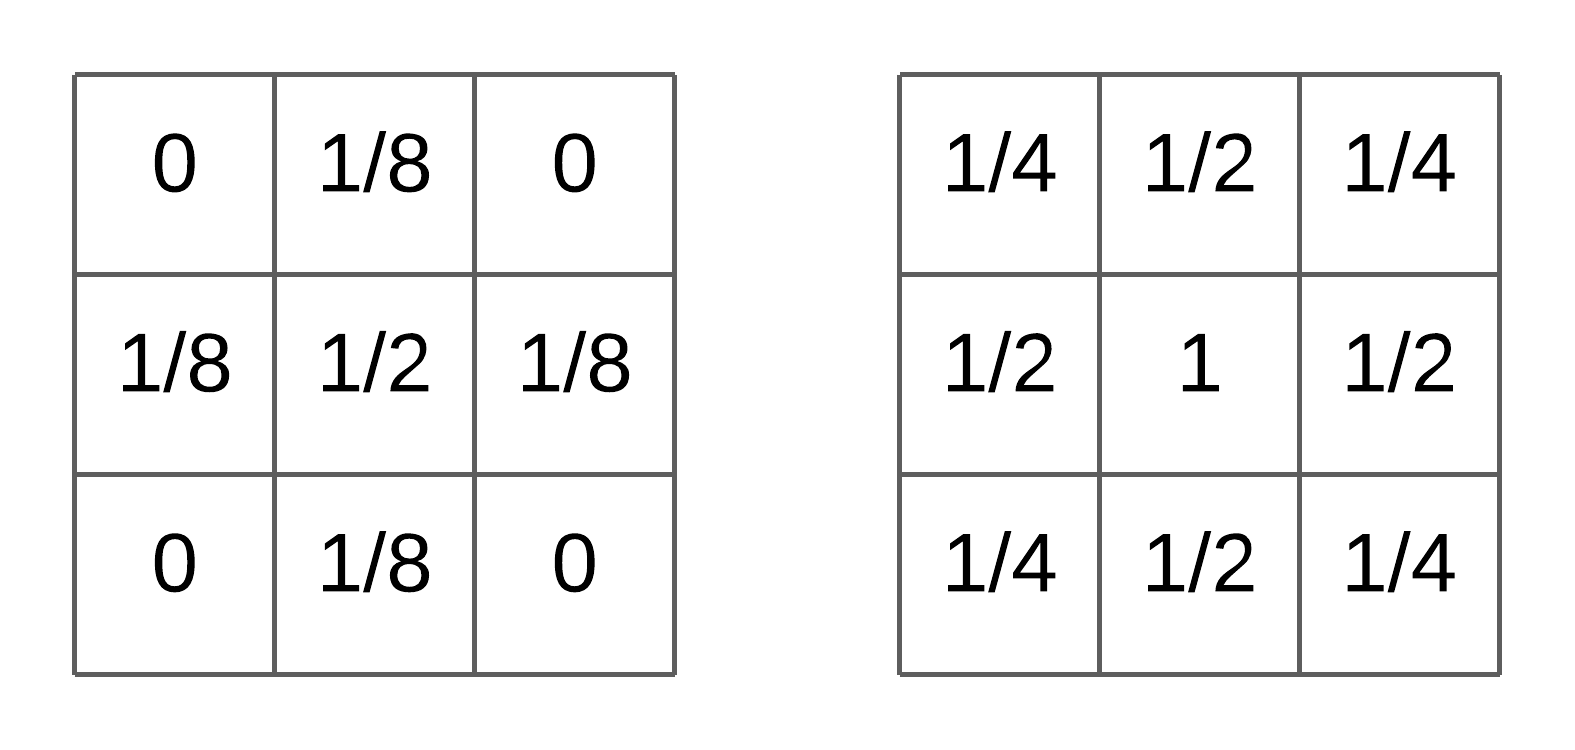
\includegraphics[width=0.4\textwidth]{../images/lvloperations.png}
    \caption{Restriction and interpolation matrices}
    \label{fig:basic}
\end{wrapfigure}

The multigrid implementation basically works by starting with the lowest grid level, i.e., the coarsest grid, and calculates a given number of iterations to get the first basic result. It then performs an interpolation operation where the result of the lower grid level is transformed to fit in the finer grid level. This can be done in several different ways but the chosen here – an operation called bilinear interpolation - is where the value of a coarser point is copied into the corresponding fine grid points, half its value is copied into the four immediate neighbours of the fine grid point and a quarter of its value is copied into the other remaining neighbors. This means that a finer level grid point that is between two coarser grid points gets half its value from each of the coarser grid points, and a fine grid point that is in the center of a square of four coarse grid points gets one quarter of its value from each of the coarse grid points(see Figure 2).

Restriction is the operation when going from a finer grid level to a coarser one – the opposite of interpolation. This means, in this implementation, that the result calculated on the finer grid level is restricted to a grid in which the points are twice as far apart. The restricting operator, because of that, works by enabling each coarser grid point to get half its initial value from the corresponding fine grid point and the other half from the sum of one-eighth of the values of each of the four nearest neighbours of the fine grid point(see Figure 2). This cycle of going up and down between levels and doing calculations on each level improves the accuracy of the calculations in a fast way since it makes calculations on the coarser grid several times before it first moves up to a finer grid level and hence yields much better initial values for the finer grid in a shorter amount of time. They also converge much more rapidly than the basic iterative methods but are much harder to program. That is because they require extensive bookkeeping in particular since they manage multiple size grids and continually restricts and interpolates between them.(see Figure 3)

\begin{figure}[h!]
    \centering
    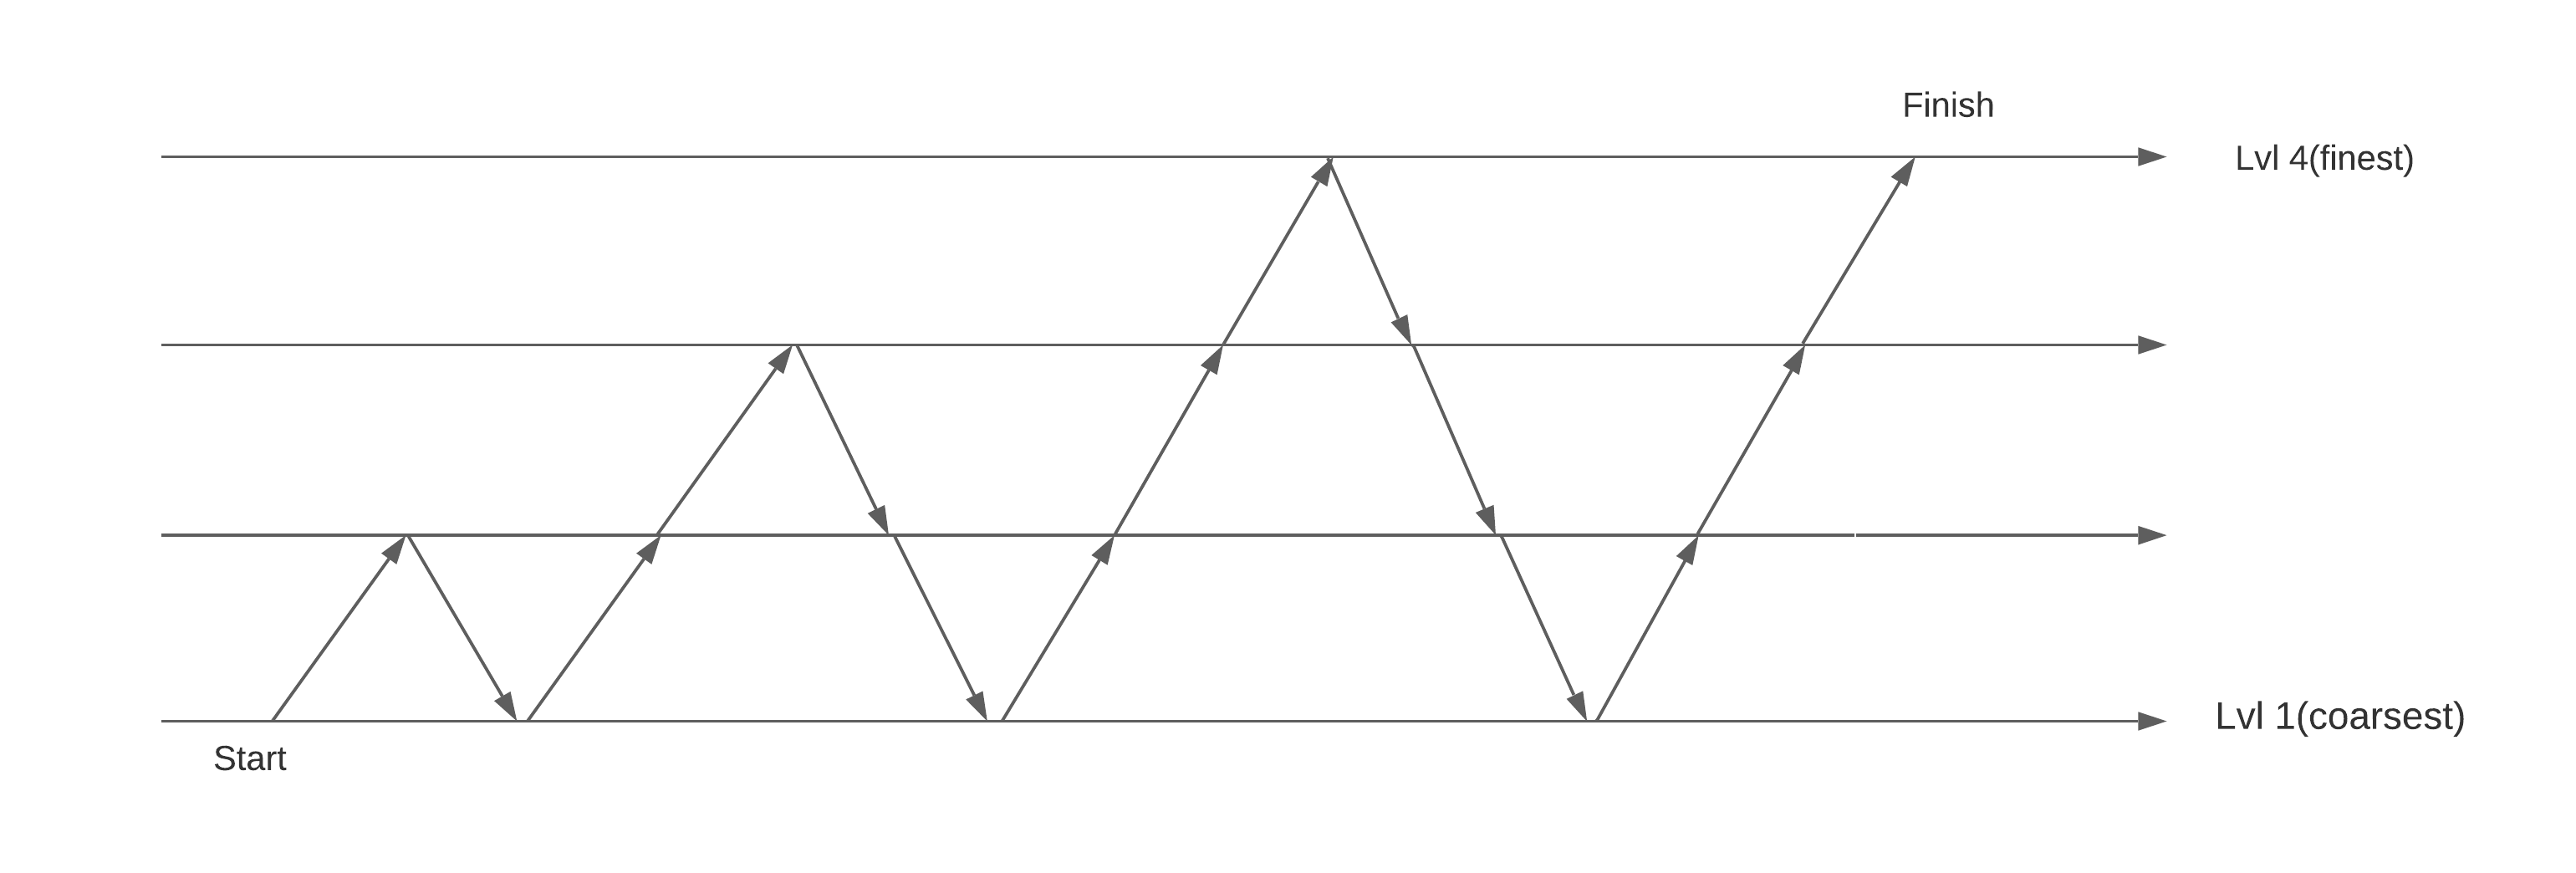
\includegraphics[width=0.8\textwidth]{../images/multigridpattern.png}
    \caption{Multigrid cycle}
    \label{fig:basic}
\end{figure}
 \newpage
 
Both sequential PDE solver versions - the basic Jacobi as well as the multigrid – were after the correctness of them had been tested parallelized with the intention of getting faster execution times and thereby better performance. This was done by using the Open MP library which is an application programming interface(API) supporting multi-platform shared memory multiprocessor programming in C which is the programming language used in the implementations. It basically is an implementation of multithreading where a primary thread forks a specified number of sub threads which identified tasks are divided among. The threads then run concurrently with the runtime environment allocating threads to different processors. To accomplish this parallelization were parts of the programs which where parallelizable identified – the tasks divided among the threads - and this were parts where a lot of independent calculations were done iteratively – basically the calculations in the grid done in the loops of the programs. The Open MP functionality were implemented at these parts to signal to the compiler that these were to be parallelized and the results of these changes are shown in the performance evaluation section.

\section{Performance Evaluation}\label{performanceevaluation}


The execution times of the sequential versions were aimed to lay around 30 seconds to get a good indication of how much speedup - a measurement of relative performance of two systems processing the same problem where a speedup larger than one is an increase in performance - was received by the parallelization. There were also two different grid sizes tested on each of the versions to see how that factor would affect the performance having multiple threads working on them. 

\begin{table}
\centering
\resizebox{\columnwidth}{!}{%
 \begin{tabular}{||c c c c c c||}

 \hline
GridSize & Iterations& Threads & Exec. Time(s) & MaxDiff & Speedup\\ [0.5ex] 
 \hline\hline
 1000 & 5000 & X & 26.80 & 0.000072 & X\\ 
 
 2000 & 1500 & X & 33.04 & 0.000240 & X\\ 
 
 1000 & 5000& 1 & 26.84 & 0.000072 & 0.99\\
  
 1000 & 5000 & 2 & 14.72 & 0.000072 & 1.82\\ 
   
 1000 & 5000 & 3 & 13.38 & 0.000072 & 2.00\\ 
    
 1000 & 5000 & 4 & 11.51 & 0.000072 & 2.33\\
 
 2000 & 1500 & 1 & 33.30 & 0.000240 & 0.99\\
  
 2000 & 1500 & 2 & 21.97 & 0.000240 & 1.50\\ 
   
 2000 & 1500 & 3 & 15.18 & 0.000240 & 2.18\\ 
    
 2000 & 1500 & 4 & 14.60 & 0.000240 & 2.26\\  

 \hline
\end{tabular}%
}
\caption{Sequential Jacobi test results}
    \label{fig:jacobi}
\end{table}

This resulted in grids with sides of 1000 and 2000 for the basic and 500 and 1000 for the lowest coarsest grid of the multigrid. 5000 and 1500 iterations were done on the small and large one respectively on the basic, and for the multigrid were 3000 and 500 iterations performed on its corresponding sizes . The iterations on the higher-level grids were restricted to four because of project instructions.


For the sequential Jacobi version,there was an execution time of 26.80 s on the small grid and 33.04 s on the large one. This improves to 11.51 s and 14.60 s when having 4 threads working on them concurrently. This means there was a speedup observed of 2.33 and 2.26 on these tests(see Table 1).

For the sequential multigrid there was an execution time of 26.09 s on the small grid and 30.21 s on the large. With implemented parallelization there were increases in performance when using four threads to 8.85 s and 11.39 s respectively. This means that there was a speedup of 2.95 on the small and 2.65 on the large one in the multigrid version(see Table 2).

\begin{table}
\centering
\resizebox{\columnwidth}{!}{%
 \begin{tabular}{||c c c c c c||}

 \hline
GridSize & Iterations& Threads & Exec. Time(s) & MaxDiff & Speedup\\ [0.5ex] 
 \hline\hline
 500 & 3000 & X & 26.09 & 0.0000898 & X\\ 
 
 1000 & 500 & X & 30.21 & 0.0002196 & X\\ 
 
 500 & 3000 & 1 & 26.14 & 0.0000898 & 0.99\\
  
 500 & 3000 & 2 & 13.56 & 0.0000898 & 1.92\\ 
   
 500 & 3000 & 3 & 10.35 & 0.0000898 & 2.52\\ 
    
 500 & 3000 & 4 & 8.85 & 0.0000898 & 2.95\\
 
 1000 & 500 & 1 & 30.25 & 0.0002196 & 0.99\\
  
 1000 & 500 & 2 & 17.39 & 0.0002196 & 1.74\\ 
   
 1000 & 500 & 3 & 13.38 & 0.0002196 & 2.26\\ 
    
 1000 & 500 & 4 & 11.39 & 0.0002196 & 2.65\\  

 \hline
\end{tabular}%
}
\caption{Sequential Multigrid test results}
\label{fig:multigrid}
\end{table}



\section{Discussion}\label{discussion}



The results of the tests were not surprising based on that parallelization through the Open MP library is an established way of increasing performance on a sequential program. That most of the increase in performance came when increasing from one thread to two thread does not seem unreasonable either since when there are two threads there are not much competition between the resources. This makes it unlikely to arise conflict with them when being loaded with tasks to perform. That the increase in speed up is a lower fraction with each number of threads added(see Figure 4) is not surprising either since the amount of work each thread performs decreases which each increase but the overhead of creating and managing the threads are the same. This mean that the overhead becomes a larger part of the overall execution time of the program. 

What is interesting though is that the speed up on the multigrid version is higher than the one on the basic Jacobi. This could be explained by that the multigrid version are working on different grid levels of granularity and since the size of the grids increases by a factor of two for each increased level. The reasoning is that the highest multigrid levels are much larger than the ones on the basic Jacobi version. This means that the threads could work for longer times on these larger grids without having the need of halting and starting over as much for each new iteration, meaning less overhead and more work done. This could indicate that parallelization works better the larger the problem sizes are, since the overhead of creating and managing new threads becomes a smaller part of the overall execution time. Deeper and more thorough tests need to be done than what fits in the scope of this paper to verify that hypothesis, but that conclusion is something which is already an established fact in the computer science world(see Gustafson’s law), so the interesting part is more likely to see that the results of this project reinforce that fact. 

\begin{figure}
\hspace{4em}
\begin{tikzpicture}
\centering
\begin{axis}[
	xlabel={Threads}, 
	ylabel={Execution time},
	y unit=s, 
	legend style={at={(0.97,0.83)},anchor=east, font=\tiny},
	grid style=dashed,
	ymajorgrids=true,
    grid style=dashed,
    cycle list name=exotic,
    xtick={1,...,4}
]
\addplot 
table[
	x expr=\coordindex+1,
	y=JacobiSmall
]{../data/jacobismall.dat};

\addplot 
table[
	x expr=\coordindex+1,
	y=JacobiLarge
]{../data/jacobismall.dat};

\addplot 
table[
	x expr=\coordindex+1,
	y=MultigridSmall
]{../data/jacobismall.dat};

\addplot 
table[
	x expr=\coordindex+1,
	y=MultigridLarge
]{../data/jacobismall.dat};

\addlegendentry{Jacobi Small}
\addlegendentry{Jacobi Large}
\addlegendentry{Multigrid Small}
\addlegendentry{Multigrid Large}
\end{axis}
\end{tikzpicture}
\caption{Performance increase when adding multiple threads}
\end{figure}


\section{Conclusion}\label{conclusion}

Iterative calculations like the Jacobi iterative solution to solve a partial differential equation like Laplace’s is a very resource heavy computation since  it consists of vast amounts of iterative calculations. How many those calculations are is based on how large the grid is on which the calculations are being performed and how those calculations are implemented. When huge calculations like on how weather, nuclear fusion/fission etc. evolves it is often desirable to increase the performance to decrease the execution time and one way of doing this is to assign the workload on several different threads working in parallel. In this paper was the Open MP library used on sequential Jacobi and multigrid implementations to attain this parallelization property, and it has shown that when implemented correctly you could get a significant speed up on these types of calculations. This has been a valuable experience to gain and the knowledge that with very little manipulation of a sequential code you could get this great increase in performance. That is a knowledge gained well worth the time invested in the project this paper is based on, and that knowledge will be taken into the future of the authors career as a computer engineer. 


\end{document}